% Chapter 1
\chapter{Definición del problema u oportunidad} % Main chapter title
\label{sec:problema} % For referencing the chapter elsewhere, use

Este capítulo debe contener la exposición general del problema. Con respecto al problema se debe responder las siguientes preguntas:
\begin{itemize}
	\item	¿Cuál es el problema u oportunidad abordado por el proyecto? ¿Es posible cuantificarlo?
	\item	¿Cuáles son las causas de la existencia de este problema u oportunidad? Haga referencia a publicaciones y/u otros antecedentes que validen estas causas.
	\item Explique cómo la memoria ayudará a abordar este problema.
	
\end{itemize}

\section{Ejemplos de latex}

Sed ullamcorper quam eu nisl interdum at interdum enim egestas. Aliquam placerat justo sed lectus lobortis ut porta nisl porttitor. Vestibulum mi dolor, lacinia molestie gravida at, tempus vitae ligula. Donec eget quam sapien, in viverra eros. Donec pellentesque justo a massa fringilla non vestibulum metus vestibulum. Vestibulum in orci quis felis tempor lacinia. Vivamus ornare ultrices facilisis. Ut hendrerit volutpat vulputate. Morbi condimentum venenatis augue, id porta ipsum vulputate in. Curabitur luctus tempus justo. Vestibulum risus lectus, adipiscing nec condimentum quis, condimentum nec nisl. Aliquam dictum sagittis velit sed iaculis. Morbi tristique augue sit amet nulla pulvinar id facilisis ligula mollis. Nam elit libero, tincidunt ut aliquam at, molestie in quam. Aenean rhoncus vehicula hendrerit.

\begin{figure}[th]
	\centering
	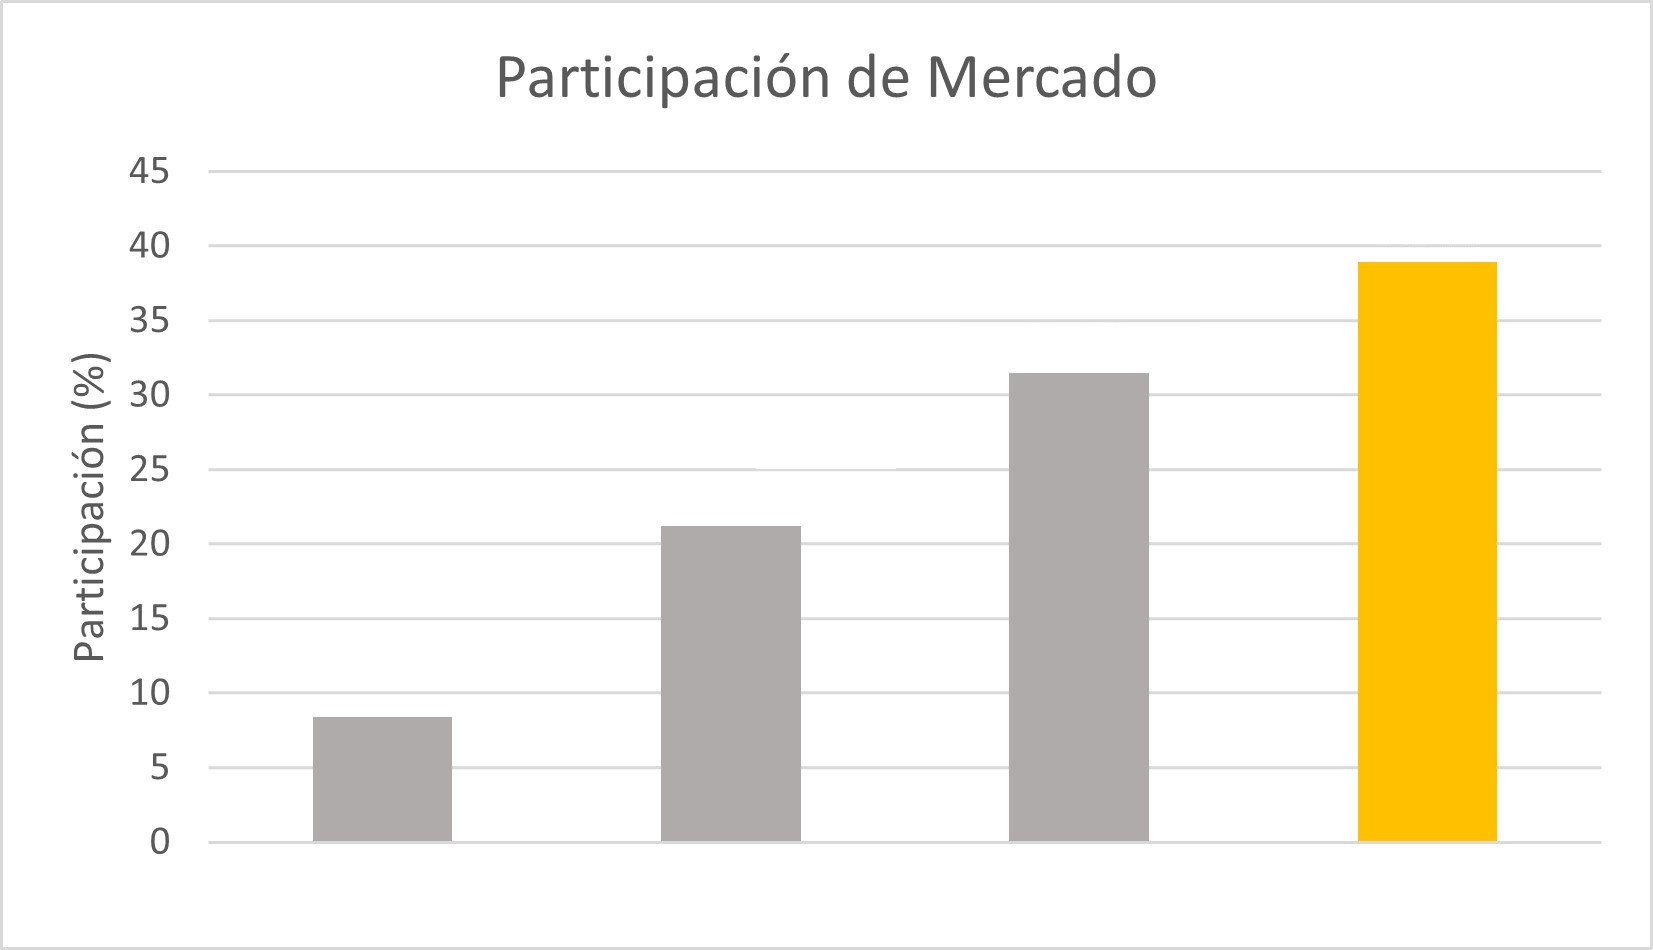
\includegraphics[width=10cm]{Figures/Ejemplo}
	\caption{Comparación de la participación de mercado entre mutuales, a enero 2020.}
	\label{fig:Ejemplo}
\end{figure}

% Citando Figura~\ref{fig:Ejemplo} de la sección~\ref{sec:problema}

Lista de items
\begin{itemize}
	\item \textbf{Componente A:} Sed ullamcorper quam eu nisl interdum at interdum enim egestas. Aliquam placerat justo sed lectus lobortis ut porta nisl porttitor. Vestibulum mi dolor, lacinia molestie gravida at, tempus vitae ligula. Donec eget quam sapien, in viverra eros. Donec pellentesque justo a massa fringilla non vestibulum metus vestibulum. Vestibulum in orci quis felis tempor lacinia. Vivamus ornare ultrices facilisis. Ut hendrerit volutpat vulputate. Morbi condimentum venenatis augue, id porta ipsum vulputate in.
	\item \textbf{Componente B:} Sed ullamcorper quam eu nisl interdum at interdum enim egestas. Aliquam placerat justo sed lectus lobortis ut porta nisl porttitor. Vestibulum mi dolor, lacinia molestie gravida at, tempus vitae ligula. Donec eget quam sapien, in viverra eros. Donec pellentesque justo a massa fringilla non vestibulum metus vestibulum. Vestibulum in orci quis felis tempor lacinia. Vivamus ornare ultrices facilisis. Ut hendrerit volutpat vulputate. Morbi condimentum venenatis augue, id porta ipsum vulputate in.
\end{itemize}

Lista enumerada
\begin{enumerate}
	\item \textbf{Componente A:} Sed ullamcorper quam eu nisl interdum at interdum enim egestas. Aliquam placerat justo sed lectus lobortis ut porta nisl porttitor. Vestibulum mi dolor, lacinia molestie gravida at, tempus vitae ligula. Donec eget quam sapien, in viverra eros. Donec pellentesque justo a massa fringilla non vestibulum metus vestibulum. Vestibulum in orci quis felis tempor lacinia. Vivamus ornare ultrices facilisis. Ut hendrerit volutpat vulputate. Morbi condimentum venenatis augue, id porta ipsum vulputate in.
	\item \textbf{Componente B:} Sed ullamcorper quam eu nisl interdum at interdum enim egestas. Aliquam placerat justo sed lectus lobortis ut porta nisl porttitor. Vestibulum mi dolor, lacinia molestie gravida at, tempus vitae ligula. Donec eget quam sapien, in viverra eros. Donec pellentesque justo a massa fringilla non vestibulum metus vestibulum. Vestibulum in orci quis felis tempor lacinia. Vivamus ornare ultrices facilisis. Ut hendrerit volutpat vulputate. Morbi condimentum venenatis augue, id porta ipsum vulputate in.
\end{enumerate}

% Citas a libro \cite{ejemploLibro} o paper~\cite{ejemploPaper}. Usted puede agregar otros tipos como journal o techincal report
\newpage

Falabella Tecnología Corporativa (FTC) actualmente posee un sistema de recomendación (Implicit Collaborative Filtering - Matrix Factorization) desarrollado en BigQuery ML (BQML) que presenta varias limitaciones importantes para el negocio: es demasiado simple para abordar la complejidad del comportamiento del cliente, tiene un bajo nivel de personalización y utiliza únicamente el identificador del cliente como dato de entrada principal, desaprovechando datos relevantes como características demográficas, comportamientos históricos y segmentaciones internas. Estas limitaciones restrigen la capacidad del sistema para generar recomendaciones personalizadas que maximicen la efectividad de las campañas de marketing.

Voy a poner las preguntas que deben responderse en esta sección para que quede más claro a que apunta cada párrafo, luego las eliminaré.

¿Cuál es el problema u oportunidad abordado por el proyecto?

De este modo, en conjunto con FTC, se busca desarrollar un sistema de recomendación basado en dominios cruzados (CDRS) que utilice los datos de las diferentes unidades de negocio del grupo Falabella, con el objetivo de mitigar el problema del \enquote{cold-start} para clientes nuevos de una determinada unidad de negocio, es decir, aquellos clientes que no cuentan con un historial previo de interacciones en dicha unidad, pero que sí poseen datos relevantes en las demás unidades de negocio del grupo. 

¿Se puede cuantificar?

Sí, la cuantificación del problema se asocia a la siguiente figura, donde se muestra principalmente, el costo de oportunidad que significaría aumentar el pool/número de clientes potenciales que se podrían captar si se implementara un sistema de recomendación basado en dominios cruzados (CDRS) que utilice datos de las diferentes unidades de negocio del grupo Falabella.

\begin{figure}[th]
	\centering
	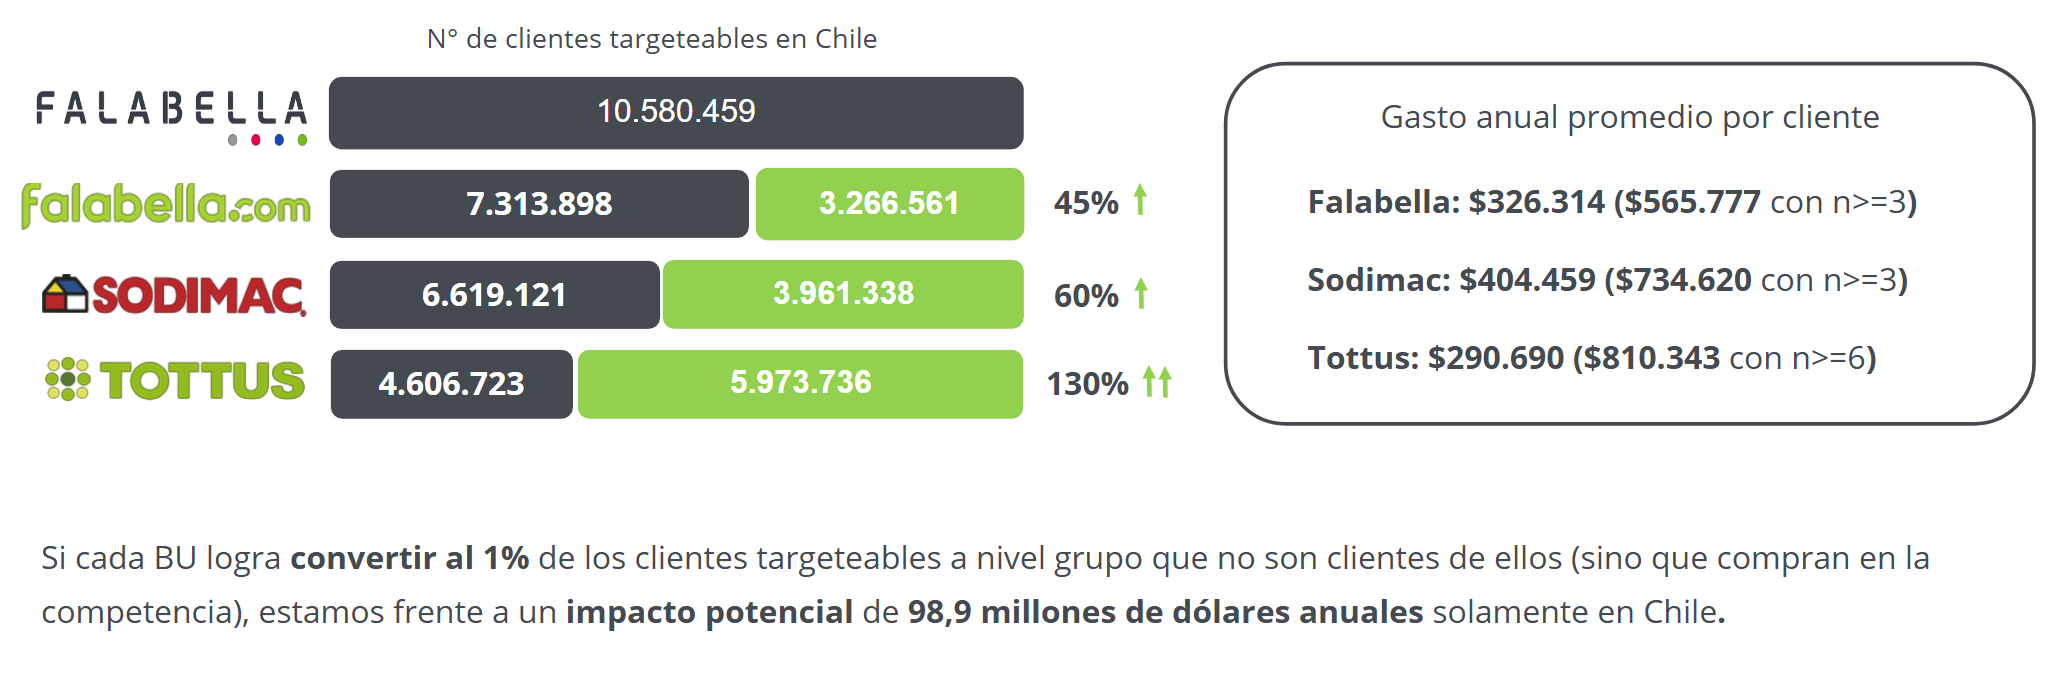
\includegraphics[width=\textwidth]{Figures/grafica Matias.png}
	\caption{Costo de oportunidad de las limitaciones del sistema de recomendación actual. Hay un par de errores menores en esta gráfica que corregiré en la versión final.}
	\label{fig:Limitaciones_Sistema_Actual}
\end{figure}

Como se puede visualizar en la figura anterior, la implementación del sistema actual está desaprovechando un mayor número de clientes potenciales, lo que se traduce en una pérdida significativa de ingresos para la empresa. Esta situación resalta la necesidad de mejorar el sistema de recomendación para captar mejor las oportunidades de venta y maximizar los beneficios comerciales. Al implementar un sistema de recomendación basado en dominios cruzados (CDRS) que utilice datos de las diferentes unidades de negocio de Falabella, se espera reducir este costo de oportunidad al aumentar la precisión y relevancia de las recomendaciones para clientes nuevos en situación de \enquote{cold-start}. Esto permitirá a la empresa aprovechar al máximo su base de clientes y mejorar su desempeño en el mercado altamente competitivo.

¿Cuáles son las causas de la existencia de de este problema u oportunidad?

No sé si acá hay que justificar las causas en base a lo determinado por FTC o si es (así como, \enquote{las causas del problema son Tangananica y Tangananá}, como lo que está en los primeros dos párrafos), más bien, justificar las causas en base a la literatura académica.

Explique cómo la memoria ayudará a abordar este problema.

No me queda claro a qué se refieren con \enquote{memoria} en este contexto. Pero asumo que se refieren a la tesis en sí misma.

En este contexto, la memoria de la tesis abordará el problema del \enquote{cold-start} en sistemas de recomendación mediante el desarrollo de un sistema basado en dominios cruzados (CDRS) que aproveche los datos de las diferentes unidades de negocio del grupo Falabella. Para ello, se desarrolló un sistema de agentes de modelos de lenguaje grande (LLM) para la tarea de relacionar distintos niveles de categorías que poseen los productos (entiéndase los niveles de categorías como, por ejemplo, \enquote{categoría: Hombre, sub-categoría: Zapatos} para la unidad de negocio de Falabella Retail), donde se agrupan y etiquetan las categorías que sean similares entre las distintas unidades de negocio. Estos nuevos atributos se pueden utilizar como características adicionales en el sistema de recomendación, permitiendo generar un modelo de sistema de recomendación que sea capaz de realizar recomendaciones más personalizadas y precisas para clientes nuevos en situación de \enquote{cold-start}, con el fin de que éstos se puedan convertir en clientes recurrentes.